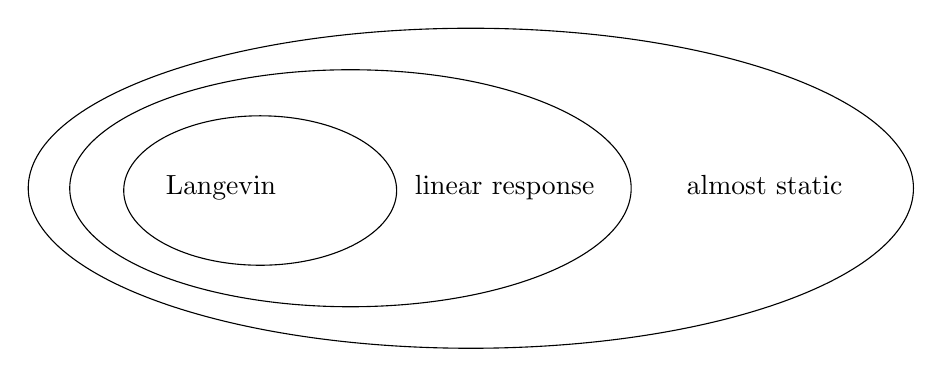
\begin{tikzpicture}[x=0.75pt,y=0.75pt,yscale=-1,xscale=1]
    %uncomment if require: \path (0,300); %set diagram left start at 0, and has height of 300
    
    %Shape: Ellipse [id:dp8043932652565831] 
    \draw   (100,185.09) .. controls (100,142.52) and (195.48,108) .. (313.25,108) .. controls (431.02,108) and (526.5,142.52) .. (526.5,185.09) .. controls (526.5,227.67) and (431.02,262.19) .. (313.25,262.19) .. controls (195.48,262.19) and (100,227.67) .. (100,185.09) -- cycle ;
    %Shape: Ellipse [id:dp3528292568204894] 
    \draw   (120,185.09) .. controls (120,153.56) and (180.55,128) .. (255.25,128) .. controls (329.95,128) and (390.5,153.56) .. (390.5,185.09) .. controls (390.5,216.63) and (329.95,242.19) .. (255.25,242.19) .. controls (180.55,242.19) and (120,216.63) .. (120,185.09) -- cycle ;
    %Shape: Ellipse [id:dp12948925288702262] 
    \draw   (146,186.19) .. controls (146,166.31) and (175.44,150.19) .. (211.75,150.19) .. controls (248.06,150.19) and (277.5,166.31) .. (277.5,186.19) .. controls (277.5,206.07) and (248.06,222.19) .. (211.75,222.19) .. controls (175.44,222.19) and (146,206.07) .. (146,186.19) -- cycle ;
    
    % Text Node
    \draw (165,177.5) node [anchor=north west][inner sep=0.75pt]   [align=left] {Langevin};
    % Text Node
    \draw (285,177.5) node [anchor=north west][inner sep=0.75pt]   [align=left] {linear response};
    % Text Node
    \draw (416,177.5) node [anchor=north west][inner sep=0.75pt]   [align=left] {almost static};
    
    
    \end{tikzpicture}
    